\documentclass{ximera}

\usepackage{epsfig}

\graphicspath{
  {./}
  {figures/}
}


\usepackage{morewrites}

%\newcounter{ccounter}
%\setcounter{ccounter}{1}
%\newcommand{\Chapter}[1]{\setcounter{chapter}{\arabic{ccounter}}\chapter{#1}\addtocounter{ccounter}{1}}

%\newcommand{\section}[1]{\section{#1}\setcounter{thm}{0}\setcounter{equation}{0}}

%\renewcommand{\theequation}{\arabic{chapter}.\arabic{section}.\arabic{equation}}
%\renewcommand{\thefigure}{\arabic{chapter}.\arabic{figure}}
%\renewcommand{\thetable}{\arabic{chapter}.\arabic{table}}

%\newcommand{\Sec}[2]{\section{#1}\markright{\arabic{ccounter}.\arabic{section}.#2}\setcounter{equation}{0}\setcounter{thm}{0}\setcounter{figure}{0}}

\newcommand{\Sec}[2]{\section{#1}}

\setcounter{secnumdepth}{2}
%\setcounter{secnumdepth}{1} 

%\newcounter{THM}
%\renewcommand{\theTHM}{\arabic{chapter}.\arabic{section}}

\newcommand{\trademark}{{R\!\!\!\!\!\bigcirc}}
%\newtheorem{exercise}{}

\newcommand{\dfield}{{\sf dfield9}}
\newcommand{\pplane}{{\sf pplane9}}

\newcommand{\EXER}{\section*{Exercises}}%\vspace*{0.2in}\hrule\small\setcounter{exercise}{0}}
\newcommand{\CEXER}{}%\vspace{0.08in}\begin{center}Computer Exercises\end{center}}
\newcommand{\TEXER}{} %\vspace{0.08in}\begin{center}Hand Exercises\end{center}}
\newcommand{\AEXER}{} %\vspace{0.08in}\begin{center}Hand Exercises\end{center}}

% BADBAD: \newcommand{\Bbb}{\bf}

\newcommand{\R}{\mbox{$\Bbb{R}$}}
\newcommand{\C}{\mbox{$\Bbb{C}$}}
\newcommand{\Z}{\mbox{$\Bbb{Z}$}}
\newcommand{\N}{\mbox{$\Bbb{N}$}}
\newcommand{\D}{\mbox{{\bf D}}}
\usepackage{amssymb}
%\newcommand{\qed}{\hfill\mbox{\raggedright$\square$} \vspace{1ex}}
%\newcommand{\proof}{\noindent {\bf Proof:} \hspace{0.1in}}

\newcommand{\setmin}{\;\mbox{--}\;}
\newcommand{\Matlab}{{M\small{AT\-LAB}} }
\newcommand{\Matlabp}{{M\small{AT\-LAB}}}
\newcommand{\computer}{\Matlab Instructions}
\newcommand{\half}{\mbox{$\frac{1}{2}$}}
\newcommand{\compose}{\raisebox{.15ex}{\mbox{{\scriptsize$\circ$}}}}
\newcommand{\AND}{\quad\mbox{and}\quad}
\newcommand{\vect}[2]{\left(\begin{array}{c} #1_1 \\ \vdots \\
 #1_{#2}\end{array}\right)}
\newcommand{\mattwo}[4]{\left(\begin{array}{rr} #1 & #2\\ #3
&#4\end{array}\right)}
\newcommand{\mattwoc}[4]{\left(\begin{array}{cc} #1 & #2\\ #3
&#4\end{array}\right)}
\newcommand{\vectwo}[2]{\left(\begin{array}{r} #1 \\ #2\end{array}\right)}
\newcommand{\vectwoc}[2]{\left(\begin{array}{c} #1 \\ #2\end{array}\right)}



\newcommand{\inv}{^{-1}}
\newcommand{\CC}{{\cal C}}
\newcommand{\CCone}{\CC^1}
\newcommand{\Span}{{\rm span}}
\newcommand{\rank}{{\rm rank}}
\newcommand{\trace}{{\rm tr}}
\newcommand{\RE}{{\rm Re}}
\newcommand{\IM}{{\rm Im}}
\newcommand{\nulls}{{\rm null\;space}}

\newcommand{\dps}{\displaystyle}
\newcommand{\arraystart}{\renewcommand{\arraystretch}{1.8}}
\newcommand{\arrayfinish}{\renewcommand{\arraystretch}{1.2}}
\newcommand{\Start}[1]{\vspace{0.08in}\noindent {\bf Section~\ref{#1}}}
\newcommand{\exer}[1]{\noindent {\bf \ref{#1}}}
\newcommand{\ans}{}
\newcommand{\matthree}[9]{\left(\begin{array}{rrr} #1 & #2 & #3 \\ #4 & #5 & #6
\\ #7 & #8 & #9\end{array}\right)}
\newcommand{\cvectwo}[2]{\left(\begin{array}{c} #1 \\ #2\end{array}\right)}
\newcommand{\cmatthree}[9]{\left(\begin{array}{ccc} #1 & #2 & #3 \\ #4 & #5 &
#6 \\ #7 & #8 & #9\end{array}\right)}
\newcommand{\vecthree}[3]{\left(\begin{array}{r} #1 \\ #2 \\
#3\end{array}\right)}
\newcommand{\cvecthree}[3]{\left(\begin{array}{c} #1 \\ #2 \\
#3\end{array}\right)}
\newcommand{\cmattwo}[4]{\left(\begin{array}{cc} #1 & #2\\ #3
&#4\end{array}\right)}

\newcommand{\Matrix}[1]{\ensuremath{\left(\begin{array}{rrrrrrrrrrrrrrrrrr} #1 \end{array}\right)}}

\newcommand{\Matrixc}[1]{\ensuremath{\left(\begin{array}{cccccccccccc} #1 \end{array}\right)}}



\renewcommand{\labelenumi}{\theenumi)}
\newenvironment{enumeratea}%
{\begingroup
 \renewcommand{\theenumi}{\alph{enumi}}
 \renewcommand{\labelenumi}{(\theenumi)}
 \begin{enumerate}}
 {\end{enumerate}\endgroup}



\newcounter{help}
\renewcommand{\thehelp}{\thesection.\arabic{equation}}

%\newenvironment{equation*}%
%{\renewcommand\endequation{\eqno (\theequation)* $$}%
%   \begin{equation}}%
%   {\end{equation}\renewcommand\endequation{\eqno \@eqnnum
%$$\global\@ignoretrue}}

%\input{psfig.tex}

\author{Martin Golubitsky and Michael Dellnitz}

%\newenvironment{matlabEquation}%
%{\renewcommand\endequation{\eqno (\theequation*) $$}%
%   \begin{equation}}%
%   {\end{equation}\renewcommand\endequation{\eqno \@eqnnum
% $$\global\@ignoretrue}}

\newcommand{\soln}{\textbf{Solution:} }
\newcommand{\exercap}[1]{\centerline{Figure~\ref{#1}}}
\newcommand{\exercaptwo}[1]{\centerline{Figure~\ref{#1}a\hspace{2.1in}
Figure~\ref{#1}b}}
\newcommand{\exercapthree}[1]{\centerline{Figure~\ref{#1}a\hspace{1.2in}
Figure~\ref{#1}b\hspace{1.2in}Figure~\ref{#1}c}}
\newcommand{\para}{\hspace{0.4in}}

\renewenvironment{solution}{\suppress}{\endsuppress}

\ifxake
\newenvironment{matlabEquation}{\begin{equation}}{\end{equation}}
\else
\newenvironment{matlabEquation}%
{\let\oldtheequation\theequation\renewcommand{\theequation}{\oldtheequation*}\begin{equation}}%
  {\end{equation}\let\theequation\oldtheequation}
\fi

\makeatother


\title{Determinants of $2\times 2$ Matrices}

\begin{document}
\begin{abstract}
\end{abstract}
\maketitle


\label{S:det2x2}

There is a simple way for determining whether a $2\times 2$ matrix $A$ is
invertible and there is a simple formula for finding $A\inv$.
\index{inverse}  First, we present the formula.  Let
\[
A=\mattwo{a}{b}{c}{d}.
\]
and suppose that $ad-bc\neq0$.  Then
\begin{equation}  \label{e:formAinv}
A\inv = \frac{1}{ad-bc} \mattwo{d}{-b}{-c}{a}.
\end{equation}
This is most easily verified by directly applying the formula for
matrix multiplication.  So $A$ is invertible when $ad-bc\neq 0$. We
shall prove below that $ad-bc$ must be nonzero when $A$ is invertible.

From this discussion it is clear that the number $ad-bc$ must be an
important quantity for $2\times 2$ matrices.  So we define:
\begin{definition}
The {\em determinant\/} \index{determinant} of the $2\times 2$
matrix $A$ is
\begin{equation}  \label{D:determinant}
\det(A) = ad - bc.
\end{equation}
\end{definition}

\begin{proposition} \label{propdet}
As a function on $2\times 2$ matrices, the determinant satisfies
the following properties.
\begin{itemize}
\item[(a)] The determinant of an upper triangular matrix is the
product of the diagonal elements. \index{matrix!upper triangular}
\item[(b)] The determinants of a matrix and its transpose are
equal. \index{matrix!transpose}
\item[(c)] $\det(AB) = \det(A)\det(B)$.
\end{itemize}
\end{proposition}

\begin{proof} Both (a) and (b) are easily verified by direct
calculation.  Property (c) is also verified by direct
calculation --- but of a more extensive sort.  Note that
\[
\left(\begin{array}{cc} a & b\\ c & d \end{array}\right)
\left(\begin{array}{cc} \alpha & \beta \\ \gamma & \delta
\end{array}\right) =
\left(\begin{array}{cc} a\alpha+b\gamma & a\beta+b\delta \\
c\alpha+d\gamma & c\beta+d\delta\end{array}\right).
\]
Therefore,
\begin{eqnarray*}
\det(AB) & = & (a\alpha+b\gamma)(c\beta+d\delta) -
     (a\beta+b\delta)(c\alpha+d\gamma)\\
& = & (ac\alpha\beta+bc\beta\gamma+ad\alpha\delta+bd\gamma\delta) \\
& & -(ac\alpha\beta+bc\alpha\delta+ad\beta\gamma+bd\gamma\delta)\\
& = & bc(\beta\gamma-\alpha\delta) +
ad(\alpha\delta-\beta\gamma) \\
& = & (ad-bc)(\alpha\delta-\beta\gamma) \\
& = & \det(A)\det(B),
\end{eqnarray*}
as asserted.   \end{proof}

\begin{corollary}  \label{C:2x2invert} \index{invertible}
A $2\times 2$ matrix $A$ is invertible if and only if $\det(A)\neq 0$.
\end{corollary}

\begin{proof}  If $A$ is invertible, then $AA\inv = I_2$.
Proposition~\ref{propdet} implies that
\[
\det(A)\det(A\inv) = \det(I_2) = 1.
\]
Therefore, $\det(A)\neq 0$.  Conversely, if $\det(A)\neq 0$, then
\eqref{e:formAinv} implies that $A$ is invertible.  \end{proof}


\subsection*{Determinants and Area}

Suppose that $v$ and $w$ are two vectors in $\R^2$ that point in different
directions.  Then, the set of points
\[
z=\alpha v + \beta w \quad\mbox{where } 0\leq\alpha,\beta\leq 1
\]
is a parallelogram\index{parallelogram}, that we denote by $P$.
We denote the area of $P$ by $|P|$.  For example, the unit square $S$, whose
corners are $(0,0)$, $(1,0)$, $(0,1)$, and $(1,1)$, is the parallelogram
generated by the unit vectors $e_1$ and $e_2$.

Next let $A$ be a $2\times 2$ matrix and let
\[
A(P) = \{Az:z\in P\}.
\]
It follows from linearity (since $Az=\alpha Av+\beta Aw$) that $A(P)$ is the
parallelogram generated by $Av$ and $Aw$.

\begin{proposition}  \label{P:det&area}
Let $A$ be a $2\times 2$ matrix and let $S$ be the unit square.  Then 
\begin{equation}  \label{e:det&area2}
|A(S)| = |\det A|.
\end{equation}
\end{proposition}

\begin{proof}   Note that $A(S)$ is the parallelogram generated by $u_1=Ae_1$ and 
$u_2=Ae_2$, and $u_1$ and $u_2$ are the columns of $A$.  It follows that
\[
(\det A)^2=\det(A^t)\det(A)=\det(A^tA) =
\det\mattwo{u_1^tu_1}{u_1^tu_2}{u_2^tu_1}{u_2^tu_2}.
\]
Hence
\[
(\det A)^2=
\det\mattwo{||u_1||^2}{u_1\cdot u_2}{u_1\cdot u_2}{||u_2||^2} =
||u_1||^2||u_2||^2-(u_1\cdot u_2)^2.
\]
Recall that \eqref{e:areaP} of Chapter~\ref{chap:prelim} states that
\[
|P|^2 = ||v||^2||w||^2 - (v\cdot w)^2.
\]
where $P$ is the parallelogram generated by $v$ and $w$.  Therefore, 
$(\det A)^2 = |A(S)|^2$ and \eqref{e:det&area2} is verified. \end{proof}


\begin{theorem}  \label{T:det&area}
Let $P$ be a parallelogram in $\R^2$ and let $A$ be a $2\times 2$
matrix.  Then
\begin{equation} \label{e:det&area}
|A(P)| = |\det A||P|.
\end{equation}
\end{theorem}

\begin{proof}  First note that \eqref{e:det&area2} a special case of \eqref{e:det&area}, 
since $|S|=1$.   Next, let $P$ be the parallelogram generated by the (column)
vectors $v$ and $w$, and let $B=(v|w)$.  Then $P=B(S)$.  It
follows from \eqref{e:det&area2} that $|P|=|\det B|$.  Moreover,
\begin{eqnarray*}
|A(P)| & = & |(AB)(S)| \\
& = & |\det(AB)| \\
& = & |\det A||\det B| \\
& = & |\det A||P|,
\end{eqnarray*}
as desired.  \end{proof}

\EXER

\TEXER

\begin{exercise} \label{c4.9.1}
Find the inverse of the matrix
\[
\mattwo{2}{1}{3}{2}.
\]

\begin{solution}

Use \eqref{e:formAinv} to compute the inverse of the matrix,
as follows:
\[ \mattwo{2}{1}{3}{2}^{-1} = \frac{1}{4-3}\mattwo{2}{-1}{-3}{2}
= \mattwo{2}{-1}{-3}{2}. \]

\end{solution}
\end{exercise}

\begin{exercise} \label{c7.8.4}
Find the inverse of the shear matrix $\mattwo{1}{K}{0}{1}$.

\begin{solution}

\ans The inverse of the matrix is
\[
\mattwo{1}{-K}{0}{1}.
\]

\soln Note that the inverse of any $2 \times 2$ matrix is:
\[ \mattwo{a}{b}{c}{d}^{-1} = \frac{1}{ad - bc}\mattwo{d}{-b}{-c}{a}. \]


\end{solution}
\end{exercise}\index{shear}

\begin{exercise} \label{c4.9.4}
Show that the $2\times 2$ matrix $A=\mattwo{a}{b}{c}{d}$ is row
equivalent to $I_2$ if and only if $ad-bc\neq 0$.  {\bf Hint:}
Prove this result separately in the two cases $a\neq 0$ and
$a=0$.

\begin{solution}

Case: $a \neq 0$.  $A$ can be row reduced as follows:
\[ \mattwo{a}{b}{c}{d} \rightarrow
\mattwo{1}{\frac{b}{a}}{c}{d} \rightarrow
\cmattwo{1}{\frac{b}{a}}{0}{\frac{ad - bc}{a}}. \]
If $ad - bc \neq 0$, then the matrix can be row reduced to $I_2$, whereas
if $ad - bc = 0$, the row reduced matrix is:
\[ \mattwo{1}{\frac{b}{a}}{0}{0} \]
which cannot be reduced further and is not row equivalent to $I_2$.

Case: $a = 0$.  If either $c = 0$ or $b = 0$, then the resulting matrices,
\[ \mattwo{0}{b}{0}{d} \AND \mattwo{0}{0}{c}{d} \]
respectively, are not row equivalent to $I_2$, and $ad - bc = 0 - 0 = 0$.
If $c \neq 0$ and $b \neq 0$, then the matrix can be row reduced:
\[ \mattwo{0}{b}{c}{d} \rightarrow
\mattwo{c}{d}{0}{b} \rightarrow \mattwo{1}{\frac{d}{c}}{0}{b} \]
which is row equivalent to $I_2$.  So $A$ is indeed row equivalent
to $I_2$ if and only if $ad - bc \neq 0$.

\end{solution}
\end{exercise}

\begin{exercise} \label{c4.9.5}
Let $A$ be a $2\times 2$ matrix having integer entries.  Find a
condition on the entries of $A$ that guarantees that $A\inv$ has
integer entries.

\begin{solution}

\ans The matrix $A^{-1}$ has integer entries when $|ad - bc| = 1$.

\soln By \eqref{e:formAinv},
\[
A^{-1} = \frac{1}{ad-bc}\mattwo{d}{-b}{-c}{a}.
\]
So, in order for $A^{-1}$ to have integer entries, $\frac{1}{ad-bc}$
must be an integer.  Since $a$, $b$, $c$, and $d$ are integers,
$\frac{1}{ad - bc}$ is an integer only if $|ad - bc| = 1$.


\end{solution}
\end{exercise}

\begin{exercise} \label{c6.4.4}
Let $A$ be a $2\times 2$ matrix and assume that $\det(A)\neq 0$.
Then use the explicit form for $A\inv$ given in \eqref{e:formAinv}
to verify that
\[
\det(A\inv) = \frac{1}{\det(A)}.
\]

\begin{solution}

Verify by computation:
\[ \det(A^{-1}) = \frac{a}{\det(A)}\frac{d}{\det(A)} -
\frac{-b}{\det(A)}\frac{-c}{\det(A)} = \frac{ad - bc}{(\det(A))^2} =
\frac{1}{\det(A)}. \]

\end{solution}
\end{exercise}

\begin{exercise} \label{c7.8.3}
Sketch the triangle whose vertices are $0$, $p=(3,0)^t$, and
$q=(0,2)^t$; and find the area of this triangle.  Let
\[
M=\mattwo{-4}{-3}{5}{-2}.
\]
Sketch the triangle whose vertices are $0$, $Mp$, and $Mq$; and
find the area of this triangle.

\begin{solution}

\ans Let $T$ be the triangle whose vertices are $0$, $p$, and $q$, and
let $U$ be the triangle whose vertices are $0$, $Mp$ and $Mq$.  Then
$A_T = 3$ is the area of $T$, and $A_U = 69$ is the area of $U$.

\soln Use the formula for the area of a triangle to compute
$A_T = \frac{1}{2}(3)(2) = 3$.  Then, use Theorem~\ref{T:det&area} to
compute
\[
A_U = |\det{M}|A_T = 23(3) = 69.
\]
Figure~\ref{c7.8.3} shows triangles $T$ and $U$.

\begin{figure}[htb]
		\centerline{%
		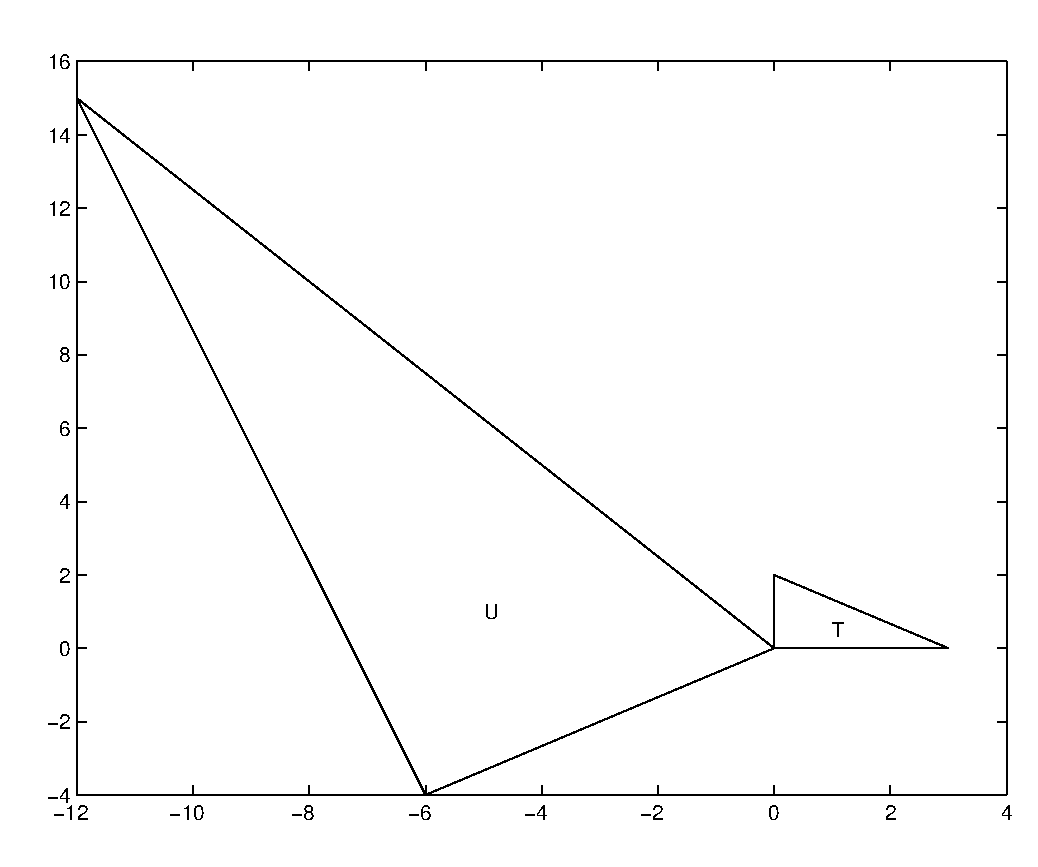
\includegraphics[width=3.0in]{exfigure/7-8-3.eps}}
	\exercap{c7.8.3}
\end{figure}

\end{solution}
\end{exercise}

\begin{exercise} \label{c7.8.4A}
Cramer's rule \index{Cramer's rule} provides a method based on determinants 
for finding the unique solution to the linear equation $Ax=b$ when $A$ is 
an invertible matrix.  More precisely, let $A$ be an invertible $2\times 2$ 
matrix and let $b\in\R^2$ be a column vector. Let $B_j$ be the $2\times 2$ 
matrix obtained from $A$ by replacing the $j^{th}$ column of $A$ by the vector 
$b$.  Let $x=(x_1,x_2)^t$ be the unique solution to $Ax=b$. Then Cramer's rule
states that 
\begin{equation}  \label{E:cramer}
x_j = \frac{\det(B_j)}{\det(A)}.
\end{equation}
Prove Cramer's rule.  {\bf Hint:}  Write the general system of two equations in 
two unknowns as
\begin{eqnarray*}
a_{11}x_1+a_{12}x_2 & = & b_1\\
a_{21}x_1+a_{22}x_2 & = & b_2.
\end{eqnarray*}
Subtract $a_{11}$ times the second equation from $a_{21}$ times the first 
equation to eliminate $x_1$; then solve for $x_2$, and verify \eqref{E:cramer}.  
Use a similar calculation to solve for $x_1$. 

\begin{solution}

The general system of linear equations in two unknowns is:
\begin{eqnarray*}
a_{11}x_1+a_{12}x_2 & = & b_1\\
a_{21}x_1+a_{22}x_2 & = & b_2.
\end{eqnarray*}
Subtract $a_{11}$ times the $2^{nd}$ equation from $a_{21}$ times the $1^{st}$ 
equation to eliminate $x_1$ and obtain
\[
(a_{21}a_{12}-a_{11}a_{22})x_2 = (a_{21}b_1-a_{11}b_2).
\]
Therefore
\[
x_2 =  \frac{a_{21}b_1-a_{11}b_2}{a_{21}a_{12}-a_{11}a_{22}}
= \frac{\det(B_2)}{\det(A)}.
\]
A similar argument works for $x_1$.

\end{solution}
\end{exercise}

\noindent In Exercises~\ref{c7.8.4B} -- \ref{c7.8.4C} use Cramer's 
rule~\eqref{E:cramer} to solve the given system of linear 
equations.
\begin{exercise} \label{c7.8.4B}
Solve \qquad $\begin{array}{rcl} 2x+3y & = & 2 \\ 3x - 5y & = & 1 \end{array}$ 
\qquad for $x$.

\begin{solution}
\ans  $x=\frac{13}{19}$.

\soln By Cramer's rule (see \eqref{E:cramer}),
\[
x = \det\mattwo{2}{3}{1}{-5}\left/\det\mattwo{2}{3}{3}{-5}=\frac{-13}{-19}\right..
\]
 

\end{solution}
\end{exercise} 
\begin{exercise} \label{c7.8.4C}
Solve \qquad
$\begin{array}{rcl} 4x-3y & = & -1 \\ x + 2y & = & 7 \end{array}$ 
\qquad for $y$.

\begin{solution}
\ans  $y=\frac{29}{11}$.

\soln By Cramer's rule (see \eqref{E:cramer}),
\[
y = \det\mattwo{4}{-1}{1}{7}\left/\det\mattwo{4}{-3}{1}{2}=\frac{29}{11}\right..
\]

\end{solution}
\end{exercise}

\CEXER

\begin{exercise} \label{c4.9.9}
Use \Matlab to choose five $2\times 2$ matrices at random and compute
their inverses.  Do you get the impression that `typically'
$2\times 2$ matrices are invertible?  Try to find a reason for
this fact using the determinant of $2\times 2$ matrices.

\begin{solution}

A randomly selected $2 \times 2$ matrix is almost always invertible.
A matrix will fail to be invertible only if the determinant of the
matrix is $0$, which is seldom the case.

\end{solution}
\end{exercise}

\noindent  In Exercises~\ref{c3.8.AA} -- \ref{c3.8.AD} use the {\sf unit 
square} icon in the program {\sf map} to test Proposition~\ref{P:det&area}, as 
follows. Enter the given matrix $A$ into {\sf map} and map the {\sf unit 
square} icon.  Compute $\det(A)$ by estimating the area of $A(S)$ --- given 
that $S$ has unit area.  For each matrix, use this numerical experiment to 
decide whether or not the matrix is invertible.
\begin{exercise}  \label{c3.8.AA}
$A=\mattwo{0}{-2}{2}{0}$.

\begin{solution}
\ans The matrix $A$ is invertible and $\det(A) = 4$.

\soln Figure~\ref{c3.8.AA} shows the {\tt map} output for this matrix.
The area of the square resulting from the map is $4$, so $|\det(A)| = 4$.

\end{solution}
\end{exercise}
\begin{exercise}  \label{c3.8.AB}
$A=\mattwo{-0.5}{-0.5}{0.7}{0.7}$.

\begin{solution}
\ans The matrix $A$ is not invertible and $\det(A) = 0$.

\soln Figure~\ref{c3.8.AB} shows the {\tt map} output for this matrix.
The square is mapped to a line, whose area is $0$, so $|\det(A)| = 0$.

\ans The matrix $A$ is invertible and $\det(A) = 1$.

\soln Figure~\ref{c3.8.AD} shows the {\tt map} output for this matrix.
The result of the map is another square of area $1$, so $|\det(A)| = 1$.

\begin{figure}[htb]
                       \centerline{%
                       \includegraphics[width=1.35in]{exfigure/3-8-AA.eps}
                       \includegraphics[width=1.35in]{exfigure/3-8-AB.eps}
                       \includegraphics[width=1.35in]{exfigure/3-8-AC.eps}
                       \includegraphics[width=1.35in]{exfigure/3-8-AD.eps}}
        \centerline{Figure~\ref{c3.8.AA}\hspace{0.8in}
        Figure~\ref{c3.8.AB}\hspace{0.8in}Figure~\ref{c3.8.AC}
        \hspace{0.8in}Figure~\ref{c3.8.AD}}

\end{solution}
\end{exercise}
\begin{exercise}  \label{c3.8.AC}
$A=\mattwo{-1}{-0.5}{-2}{-1}$.

\begin{solution}
\ans The matrix $A$ is not invertible and $\det(A) = 0$.

\soln Figure~\ref{c3.8.AC} shows the {\tt map} output for this matrix.
The square is mapped to a line, whose area is $0$, so $|\det(A)| = 0$.


\end{solution}
\end{exercise}
\begin{exercise}  \label{c3.8.AD}
$A=\mattwo{0.7071}{0.7071}{-0.7071}{0.7071}$.
\end{exercise}

\end{document}

%%% Local Variables:
%%% mode: latex
%%% TeX-master: "../linearAlgebra"
%%% End:
